\chapter{Lab6}
\begin{flushleft}

Chapter 2 Differential Calculus of Functions of One Variable

The definitions of

$$
f(x_0-) =  \lim_{x \rightarrow x_0-} f(x), f(x_0+) =  \lim_{x \rightarrow x_0+} f(x), and  \lim_{x \rightarrow x_0} f(x)
$$


do not involve $f(x_0)$ or even require that it be defined. However, the case where $f(x_0)$ is
defined and equal to one or more of these quantities is important

\begin{definition}\label{d219}


\begin{enumerate}[label=\alph*.]
\item  We say that $f$ is continuous at $x_0$ if $f$ is defined on an open interval$(a, b)$ containing
$x_0$ and $ \lim_{x \rightarrow x_0} f(x) = f(x_0).$

\item  We say that $f$ is continuous from the left at $x_0$ if $f$ is defined on an open interval
$(a, x0)$ and $f(x_0-) = f(x_0).$
\item  We say that $f$ is continuous from the right at $x_0$ if f is defined on an open interval
$(x0, b)$ and $f(x_0+) = f(x_0).$
\end{enumerate}
\end{definition}



The following theorem provides a method for determining whether these definitions are
satisfied. The proof, which we leave to you (Exercise 1), rests on \ref{d221} \ref{d219}


\begin{theorem}\label{t219}
\begin{enumerate}[label=\alph*.]
\item  A function $f$ is continuous at $x_0$ if and only if $f$ is defined on an open interval $(a, b)$
containing $x_0$ and for each $ \epsilon  > 0$ there is a $\delta  > 0$ such that




\begin{equation}\label{formula1}
| f(x) - f (x_0) | < \epsilon
\end{equation}

whenever $\mid x - x_0 \mid < \delta$
\item  A function $f$ is continuous from the right at $x_0$ if and only if $f$ is defined on an
interval $(x0, b)$ and for each $ \epsilon  > 0$ there is a$\delta  > 0$ such that \ref{formula1} holds whenever
$x0 \leq x < x0 + \delta $
\item 
 A function $f$ is continuous from the left at $x_0$ if and only if $f$ is defined on an interval
$[x_0,b)$ and for each $\epsilon > 0$ 
there is a $\delta > 0$ such that \ref{formula1} holds whenever $x_0 - \delta <x \leq x_0 .$

\end{enumerate}
\end{theorem}

From \ref{d221} and \ref{t219}, $f$ is continuous at $x_0$ if and only if 

$$
f(x_0-) = f(x_0+)=f(x_0)
$$


or, equivalently, if and only if it is continuous from the right and left at $x_0$ (Exercise 2).


\textbf{Example 2.2.1} Let $f$ be defined on $[0,2] $

$$
f(x) =\begin{cases}x^2 & 0 \leq x < 1, \\ x+1 & 1 \leq  x \leq 2 \end{cases} 
$$

\newpage



Section 2.2 Continuity 55

 then


\begin{align*}
            f(0+) = 0 = f(0),\\
f(1-) = 1 \neq f(1) = 2 ,\\
f(1+) = 2 = f(1),\\
f(2-) = 3 = f(2). 
\end{align*}






Therefore, $f$ is continuous from the right at 0 and 1 and continuous from the left at 2, but
not at 1. If$ 0 < x, x0 < 1$, then


 \begin{align*}
|f(x) = f(x_0)| = |x^2 - x_0^2| = |x-x_0| |x+x_0| \\
\leq 2 |x-x_0| <  \epsilon   if  |x -x_0| < \epsilon /2.
  \end{align*}



Hence, $f$ is continuous at each $x_0$ in $(0, 1)$. If $1 < x, x_0 < 2$ then

\begin{align*}
|f(x) - f(x_0)| = |(x+1)-(x_0+1) = | x+x_0|  \\
< \epsilon \ \   if \ \   |x -x_0| < \epsilon .
\end{align*}

 
Hence, $f$ is continuous at each $x_0$ in $(1,2)$





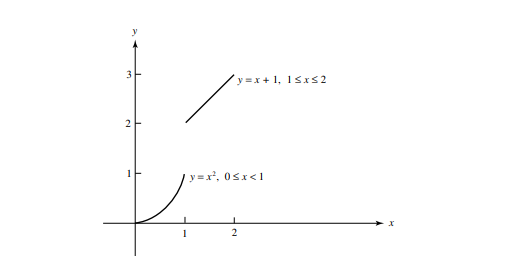
\includegraphics{labs/Figure.PNG}\\
\centering \textbf{Figure 2.2.1} 

\begin{definition}\label{d221}

 A function $f$ is continuous on an open interval $(a, b)$ if it is continuous at every point in $(a, b)$ If, in addition, 

\begin{equation}\label{formula2}
f(b-) = f(b)
\end{equation}
or

\begin{equation}\label{formula3}
f(a+) = f(a)
\end{equation}
\end{definition}

\end{flushleft}



